\documentclass[english,11pt]{article}


\oddsidemargin=-.25in
\evensidemargin=-.25in
\textwidth=7in
\topmargin=-.5in
\textheight=9in
\parindent=0in

%\usepackage[math]{iwona}
%\usepackage{cmbright}
\usepackage{setspace}
\usepackage{amssymb,amsmath}
\usepackage{graphicx}
\usepackage{fancyhdr}
\usepackage{multicol}
\usepackage{enumerate}
\usepackage{float}
%\usepackage{wrapfig}
%\usepackage{tikz}
%\usepackage{verbatim}
\usepackage{subfig}

\newcommand{\qed}{\hfill \mbox{\raggedright \rule{.065in}{.13in}}}
\newcommand{\itg}{\mathbb{Z}}
\newcommand{\rat}{\mathbb{Q}}
\newcommand{\nat}{\mathbb{N}}
\newcommand{\comp}{\mathbb{C}}
\newcommand{\real}{\mathbb{R}}
\newcommand{\bddfunc}{\xrightarrow{\text{bdd}}}
\newcommand{\inter}{\mathbb{I}}
\newcommand{\parti}{\mathcal{P}}
\newcommand{\rsharp}{\mathbb{R}^{\#}}
\renewcommand{\iff}{\longleftrightarrow}
\newcommand{\bprove}{\textbf{Prove: }}
\newcommand{\bproof}{\textbf{Proof: }}
\newcommand{\rank}[1]{\text{rank}\right(#1\left)}
\newcommand{\dist}{\text{dist}}
\newcommand{\tail}[1]{\text{tail}_{#1}}
\newcommand{\re}[1]{\text{Re}\left(#1\right)}
\newcommand{\im}[1]{\text{Im}\left(#1\right)}
\newcommand{\tab}{\hspace*{2em}}
\newcommand{\Prb}{\text{Pr}}
\newcommand{\Est}{\hat{\theta}}
\newcommand{\tbf}{\textbf}
\newcommand{\tit}{\textit}
\newcommand{\ent}{\vskip 12pt}
\newcommand{\toprob}{\xrightarrow{P}}
\newcommand{\todist}{\xrightarrow{\mathcal{L}}}
\newcommand{\mean}{\overline}
\newcommand{\iid}{\overset{iid}{\sim}}
\newcommand{\cov}{\text{Cov}}
\newcommand{\var}{\text{Var}}
\thispagestyle{fancy}
\lhead{ST 599}
\chead{}
\rhead{Kevin Park}
\renewcommand{\headrulewidth}{.25pt}
%%% Here we set the spacing  %%%%
\onehalfspace
%% This gets rids of the numbers %%%%
\setcounter{secnumdepth}{-1} 

\begin{document}
\textbf{Spectral Clustering}\\
Another method we apply is spectral clustering to determine the different clusters in our training set of the astronomy data. We did not perform any form of dimensional reduction besides removing the covariates (around 10) that largely contained 0 entries or NAs.  
\begin{center}
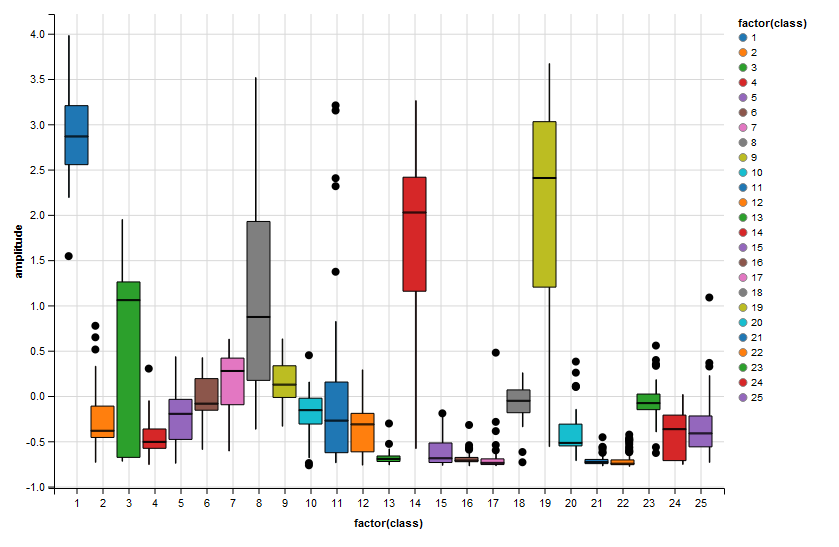
\includegraphics[scale=0.38]{estimated.png}
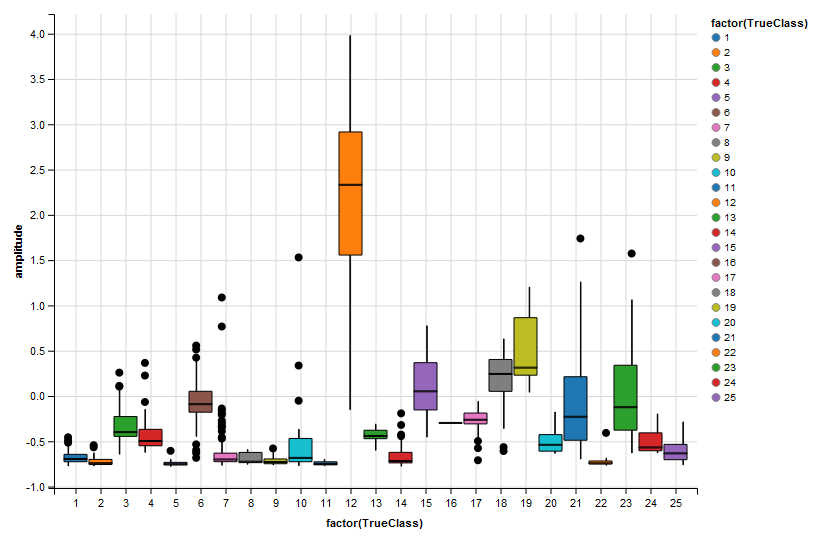
\includegraphics[scale=0.38]{trueclass.png}
\end{center}
On the left represents the estimated distribution of the clusters and on the right represents the true distribution of stars with respect to the amplitude data. 
Compared to the other methods, spectral clustering more evenly distributed the sizes between the 25 groups. An important note, the numbers along the x-axis does not represent the same star group as in the true classes. Instead it is the group designated by method from spectral clustering. 

\textbf{Issues with Spectral Clustering}\\
However, there is much difficulty in running spectral clustering on larger data set of the astronomy data, such as the low noise data set. The amount of computational time increases dramatically as the dimension size becomes larger. Spectral clustering need to first compute a the kernel matrix, that is the distances between all possible pairs. Moreover, we need to compute the eigenvalues of the kernel matrix. 

\textbf{Additional questions:}\\
To perform a spectral clustering on the larger data set, we may consider in selecting a random subset (i.e., 10\% or 20\%) of the data and apply the method of spectral clustering. Perhaps repeat this method multiple times and measure how often each which cluster group the individual observations are assigned. 
 

\end{document}